\begin{figure}[htbp]

\begin{center}
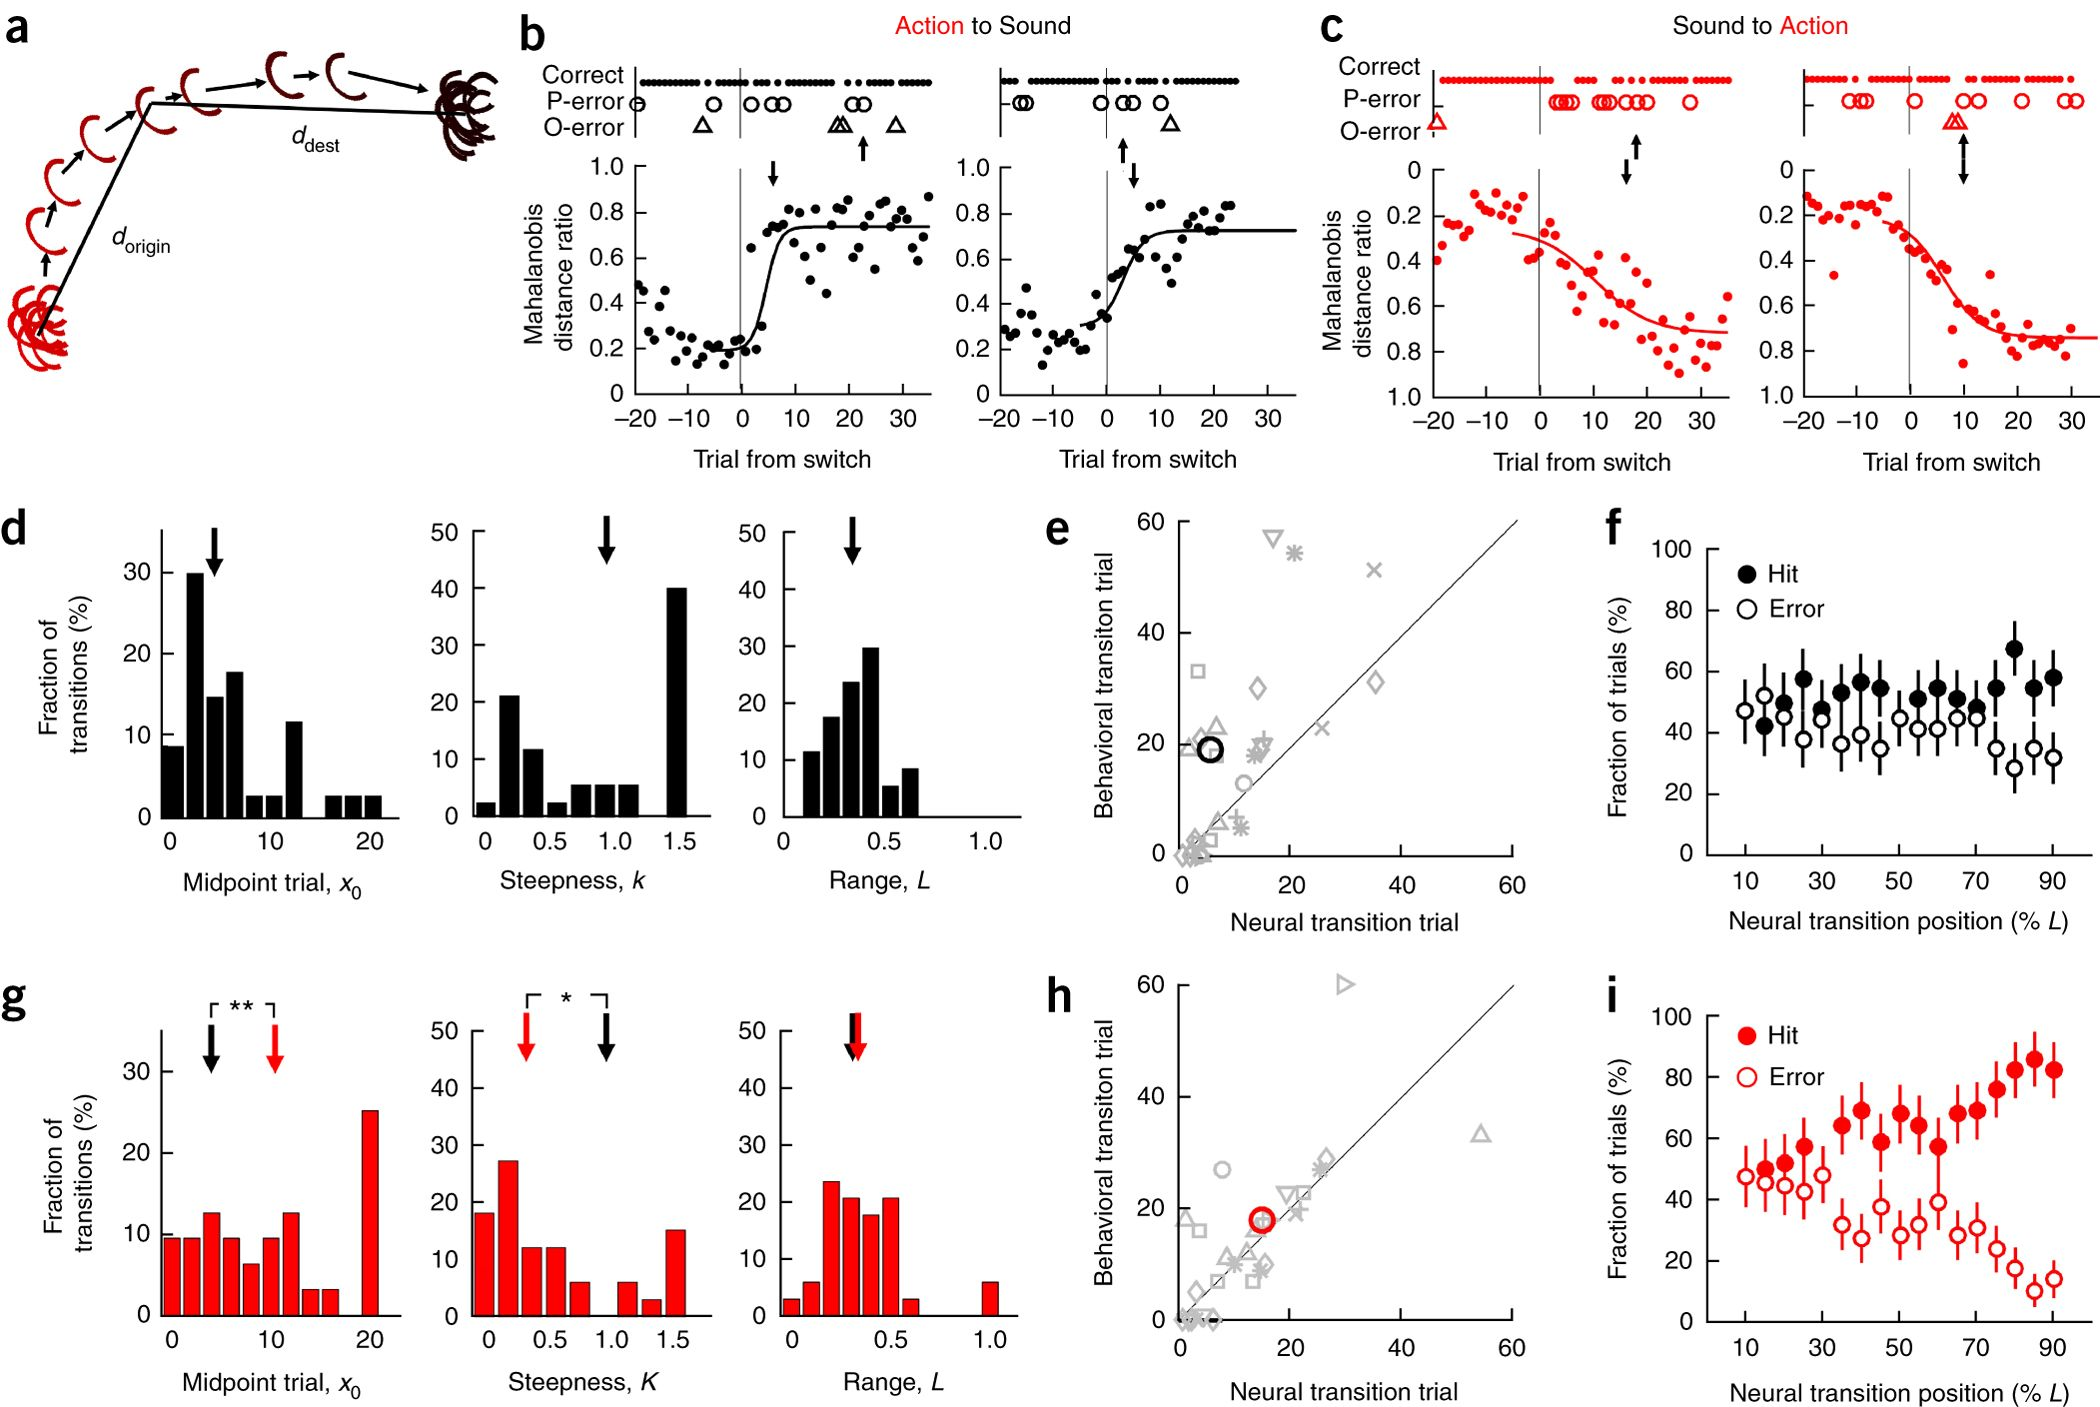
\includegraphics[width=\textwidth]{Figures/Chapter3/NN_fig4} 
\end{center}

\caption[Ensemble activity transitioned earlier and more abruptly following switch to sound rule]
{Transitions in ensemble activity occurred earlier and more abruptly following switch to sound rule. (a) Schematic illustrating ensemble activity dynamics around a block switch. Each curved line represents a single-trial neural trajectory deduced from Ca$^{2+}$-imaging data. When contingencies switch, neural trajectories move within the representational space. Trial-by-trial location of ensemble activity patterns was determined by calculating a ratio of Mahalanobis distances, $\frac{d_{origin}}{d_{origin} + d_{dest}}$, where $d_{origin}$ and $d_{dest}$ are the Mahalanobis distances from the neural trajectory of the current trial to those of the 20 trials pre-switch in the last and current blocks, respectively. (b) Two switches from action to sound blocks. Top, trial outcomes: correct (filled circles), perseverative error (P-error, open circles), and other error (O-error, open triangles). Bottom, trial-by-trial location of ensemble activity patterns. Dots, Mahalanobis distance ratios for individual trials. Lines, fit to logistic function. Up arrows, behavioral transition trials. Down arrows, neural transition trials. (c) Same as \emph{b} for two switches from sound to action blocks. Vertical axis is inverted for presentation purposes. (d) Parameters extracted by fitting action-to-sound neural transitions with the logistic function. Arrows, median values. (e) Neural transition trials plotted against behavioral transition trials (see Methods) for action-to-sound switches. Each symbol represents one block switch. Symbol shapes denote different sessions (see Supplementary Fig. \ref{fig:NN_figS6}). Large circle, median value. (f) Mean hit and error rates at the behavioral trial corresponding to specific neural transition locations as estimated by the logistic fit for each action-to-sound transition. Circles, $\mathit{mean}\pm\mathit{SEM}$. (g–i) Same as \emph{d--f} for switches from sound to action blocks; red arrows, median values; black arrows in \emph{g} shown for comparison with \emph{c}. Wilcoxon rank-sum test: for midpoint trial $x_0$, $p = 0.007$, $z = 2.70$; for steepness $k$, $p = 0.03$, $z = -2.17$; *$p < 0.05$; **$p < 0.01$. Difference in range $L$ was not significant (median $L$, sound: 0.36, action: 0.38; $p = 0.8$, $z = 0.28$). Rightmost bar of the histogram includes all instances above the range. $n = 33$ action-to-sound and 35 sound-to-action switches from 9 sessions from 5 mice.}

\label{fig:NN_fig4}
\end{figure}